\documentclass[]{article} 
\usepackage[czech]{babel}
\usepackage[IL2]{fontenc}
\usepackage[utf8]{inputenc}
\usepackage[usenames,dvipsnames]{color}
\usepackage{graphicx}
\usepackage{colortbl}
\usepackage{stmaryrd}
\usepackage{pifont}
\usepackage{hyperref}
\usepackage{pdfpages}

\newcommand\fnurl[2]{%
  \href{#2}{#1}\footnote{\url{#2}}%
}

\oddsidemargin=-5mm
\evensidemargin=-5mm\marginparwidth=.08in \marginparsep=.01in
\marginparpush=5pt\topmargin=-15mm\headheight=12pt
%\headsep=25pt\footheight=12pt \footskip=30pt\textheight=25cm
\textwidth=17cm\columnsep=2mm
\columnseprule=1pt\parindent=15pt\parskip=2pt

\begin{document}
\begin{center}
\bf Semestralni projekt MI-PAP 2011/2012:\\[5mm]
    Kostra grafu s minimálním stupněm\\[5mm] 
       Luboš Krčál\\
       Jiří Kopecký\\
       [2mm]
FIT CVUT, Kolejní 550/2, 160 00 Praha 6\\[2mm]
Pokr. z MI-PAR (Luboš Krčál a Alena Varkočková)\\[10mm]
\today
\end{center}

\section{Definice problému a popis sekvenčního algoritmu}

\subsection{Vstupní data}
$G(V,E)$ = jednoduchý neorientovaný neohodnocený k-regulární graf o~$n$ uzlech a $m$ hranách\\
$n$ = přirozené číslo představující počet uzlů grafu $G$, $n \geq 5$\\
$k$ = přirozené číslo řádu jednotek představující stupeň uzlu grafu $G$, $n \geq k \geq 3$; $n$ a $k$~nejsou současně obě liché\\
\\
Doporučení pro generování $G$:\\
\\
Usage: Graf byl generován pomocí poskytnutého \href{''https://edux.fit.cvut.cz/courses/MI-PAR/labs/zadani_semestralnich_praci/generator_grafu'}{'generátoru'} grafu s~volbou typu grafu \texttt{"-t REG"}, který vygeneruje souvislý neorientovaný neohodnocený graf.

\subsection{Úkol}
Nalezněte kostru grafu G (strom) s minimálním stupněm. Řešení existuje vždy, vždy lze sestrojit kostru grafu. Sekvenční algoritmus je typu BB-DFS s hloubkou prohledávaného prostoru omezenou na $|V|$. Přípustný mezistav je definovaný částečnou kostrou. Přípustný koncový stav je vytvořená kostra. Algoritmus končí po prohledání celého prostoru či při dosažení dolní meze. Cena, kterou minimalizujeme, je stupeň kostry.

\subsection{Výstupní data}
Výstupem programu je kosra grafu a její stupeň. Po informaci o stupni aktuálně nalezené kostry následuje posloupnost jednotlivých hran kostry, které jsou identifikovány čísly uzlů - počátečního a konečného. Příklad výstupu u grafu o 18 uzlech:

\begin{verbatim}
New spanning tree of degree: 3
[0->6][0->7][0->13][6->4][4->3][3->1][1->2][1->8][2->12][3->5][4->10][6->14][7->9][7->11]
[14->15][15->16][15->17]
\end{verbatim}

\subsection{Implementace sekvenčního algoritmu}
Pro reprezentaci grafu byla v sekvenčním i paralelním řešení použita grafová knihovna \fnurl{Boost Graph Library}{http://www.boost.org/doc/libs/1_48_0/libs/graph/doc/}, konkrétně třída \verb|boost::graph<std::vector, std::vector, unoriented>|.

Hledání kostry je realizováno pomocí prohledávání do hloubky (DFS). Při prohledávání jsou na stack (\verb|std::vector<dfs_state>|) ukládán vlastní struct, \verb|dfs state|. Každý stav je tedy definován pomocí čtyř iterátorů - vertex iterator, vertex iterator end, adjacency iterator a adjacency iterator end. Vertex iterátor iteruje přes uzly grafu, adjacency iterator přes všechny následovníky aktuálního uzlu. Koncové iterátory ukazují na konec prohledávaného prostoru.

Další zásobník (tentokráte \verb|std::vector<uint16_t>|) je použit pro ukládání aktuálního maximálního stupně kostry pro každý stav aktuálně uložený na zásobníku.

\section{OpenMP paralelní implementace}

\subsection{Struktura algoritmu}

Základní myšlenka sekvenčního algoritmu je zachována. Tj. procházení stavů probíhá stejným způsobem. V předem definovaném intervalu však dochází k odtrhávání stavového prostoru, který aktuální vlákno řeší. Protože stavový prostor není vyvážený, nelze nikterak určit, jaké množství stavového prostoru se odděluje. Může se tedy stát, že oddělený stavový prostor bude zcela nevalidní. Toto není překážkou.

Stavový prostor odtržený od probíhajícího výpočtu je uložen do globální fronty. Ukládá se pouze ukazatel na datovou strukturu. Tato datová struktura plně identifikuje stav výpočtu a lze z ní snadno zreprodukovat původní stav a pokračovat ve výpočtu.

\begin{verbatim}
struct kgm_task_struct
{
    uint32_t id;
    std::vector<i_dfs_state> inactiveDfsStack;
    uint16_t newVItStart;
    uint16_t newVItEnd;
    uint16_t degree;
};

typedef boost::shared_ptr<kgm_task_struct> kgm_task;
typedef std::queue<kgm_task> kgm_task_queue;
\end{verbatim}

Pokud vlákno vyčerpá svůj stavový prostor, zkusí vytáhnout další stav z globální fronty. Při selhání se vlákno přepně do neběžícího stavu. V tomto stavu pouze čeká, dokud nebude ve frontě opět nějaký úkol, nebo dokud výpočet neskončí.

Všechny výpočty probíhají v blocích. Tyto bloky končí po předdefinovaném množství navštívených stavů, nebo při vyčerpaní aktuálního stavového prostoru. Mohou tedy vzniknout slepé výpočetní větve, případně mírné zdržování ukončení výpočtu. Toto je nesrovnatelně vyváženo zredukováním režie komunikace, která tak probíhá zřídka.

\subsection{Ukončení výpočtu}

K ukončení výpočtu může dojít dvěma způsoby. První z nich je, že některý z procesů našel kostru s nejmenším možným stupněm, tedy 2. V takovém případě nastaví ukončující podmínku všem ostatním vláknům, která pří první příležitosti ukončí výpočet.

Druhou situací s jakou dojde k ukončení výpočtu je prohledání celého stavového prostoru bez nalezení nejmenšího možného řešení, tedy kostry se stupněm 2. V takovém případě procesory zdetekují, že nikdo již nepracuje, frotna je prázdná, a skončí.

\subsection{Měření}

Měření probíhala na lokálním počítači pro různé úlohy a konfigurace (počet vláken). Na vstupních datech, která toto umožnila (bez optimálního řešení, prochází celý stavový prostor), jsme došli k následujícím závěrům:

\begin{itemize}
  \item CPU čas odpovídá součtu výpočetní části a režie pro komunikaci mezi vlákny. Pro 64 vlákem byl CPU čas přibližně o 50"\%" větší než při výpočtu pouze jedním vláknem.
  \item Reálný čas klesal s přibývajícími vlákny až k hranici počtu fyzických procesorů. HyperThreading se nikterak neprojevil.
  \item Škálování algoritmu: Výpočetní blok vlákna měl malý vliv na dobu běhu, pokud se pohyboval v řádu $0x100$ až do $\frac{N}{(T\cdot 0x100)}$, kde $N$ je celkový počet stavů a $T$ je počet vláken.
\end{itemize}

Jako další vhodné optimalizační experimenty lze provést změnu datových struktur sloužících k uložení stavu, případně navrhnout dynamické škálování bloků podproblémů.


\section{CUDA paralelní implementace}

\subsection{Struktura algoritmu}

Implementace prohledávání do hloubky je založena na paralelním výběru posledních stavů ze zásobníku, jejich následné expanzi a uložení následníku na zásobník. K tomuto se používá paralelní prefixový součet přes počet následníků káždého stavu. Výsledek PPS slouží jako index k ukládání těchto stavů na zásobník.

Zásobník je uložen v globální paměti, protože sdílená pamět nemá dostatečnou velikost. Jako možná výlepšení se nabízí omezení velikosti zásobníku a jeho použití pouze k vyvažování práce mezi vlákny (tak jako OpenMP řešení).

\subsection{Měření}

Testování probíhalo na GeForce 9500M GS, cuda 1.1.


\section{Závěr}

\newpage
\begin{thebibliography}{9}

\bibitem{par}
{\em Pavel Tvrdík}
       {\bf Parallel Algorithms and Computing}\\
		Vydavatelství ČVUT, 2. vydání. Duben 2009

\bibitem{edux}
{\em EDUX FIT ČVUT}
       {\bf edux.fit.cvut.cz}\\
       \url{https://edux.fit.cvut.cz/courses/MI-PAR/}, [cit. 2011-11-18]
       
\bibitem{bgl}
{\em Jeremy G. Siek, Lie-Quan Lee, Andrew Lumsdaine }
       {\bf The Boost Graph Library: User Guide and Reference Manual}\\
       
       
 \end{thebibliography}

\section{Příloha A}
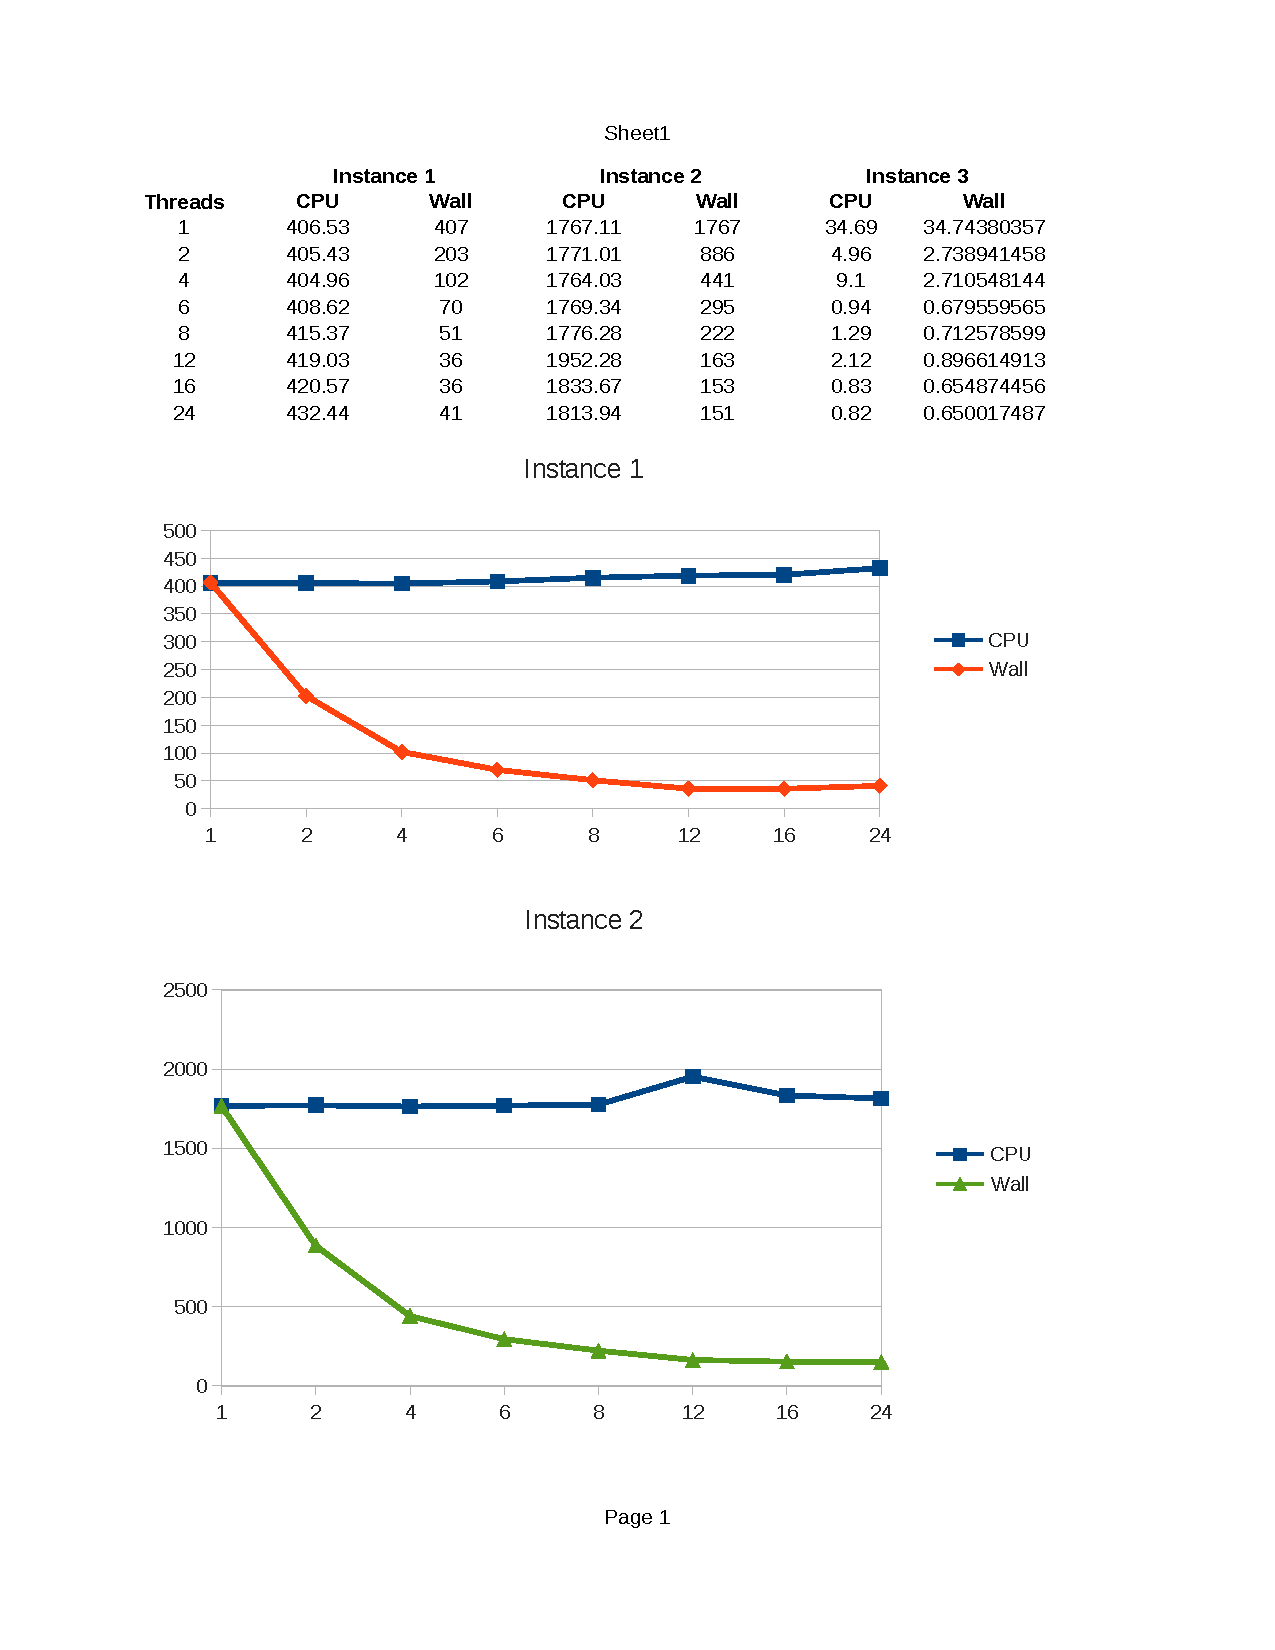
\includepdf[pages={-}]{results-omp.pdf}

\end{document}